\section{中断到键盘输入的全链路验证}

\begin{keyidea}
中断不把设备数据“推入 C++ 函数”。设备先把事实保存在自己的寄存器或缓冲区，
再用 IRQ 请求 CPU 改变控制流；处理函数必须读取真正的数据来源、确认中断、
更新有界软件状态，最后恢复被打断的现场。
\end{keyidea}

\begin{sidewaysfigure}[p]
  \centering
  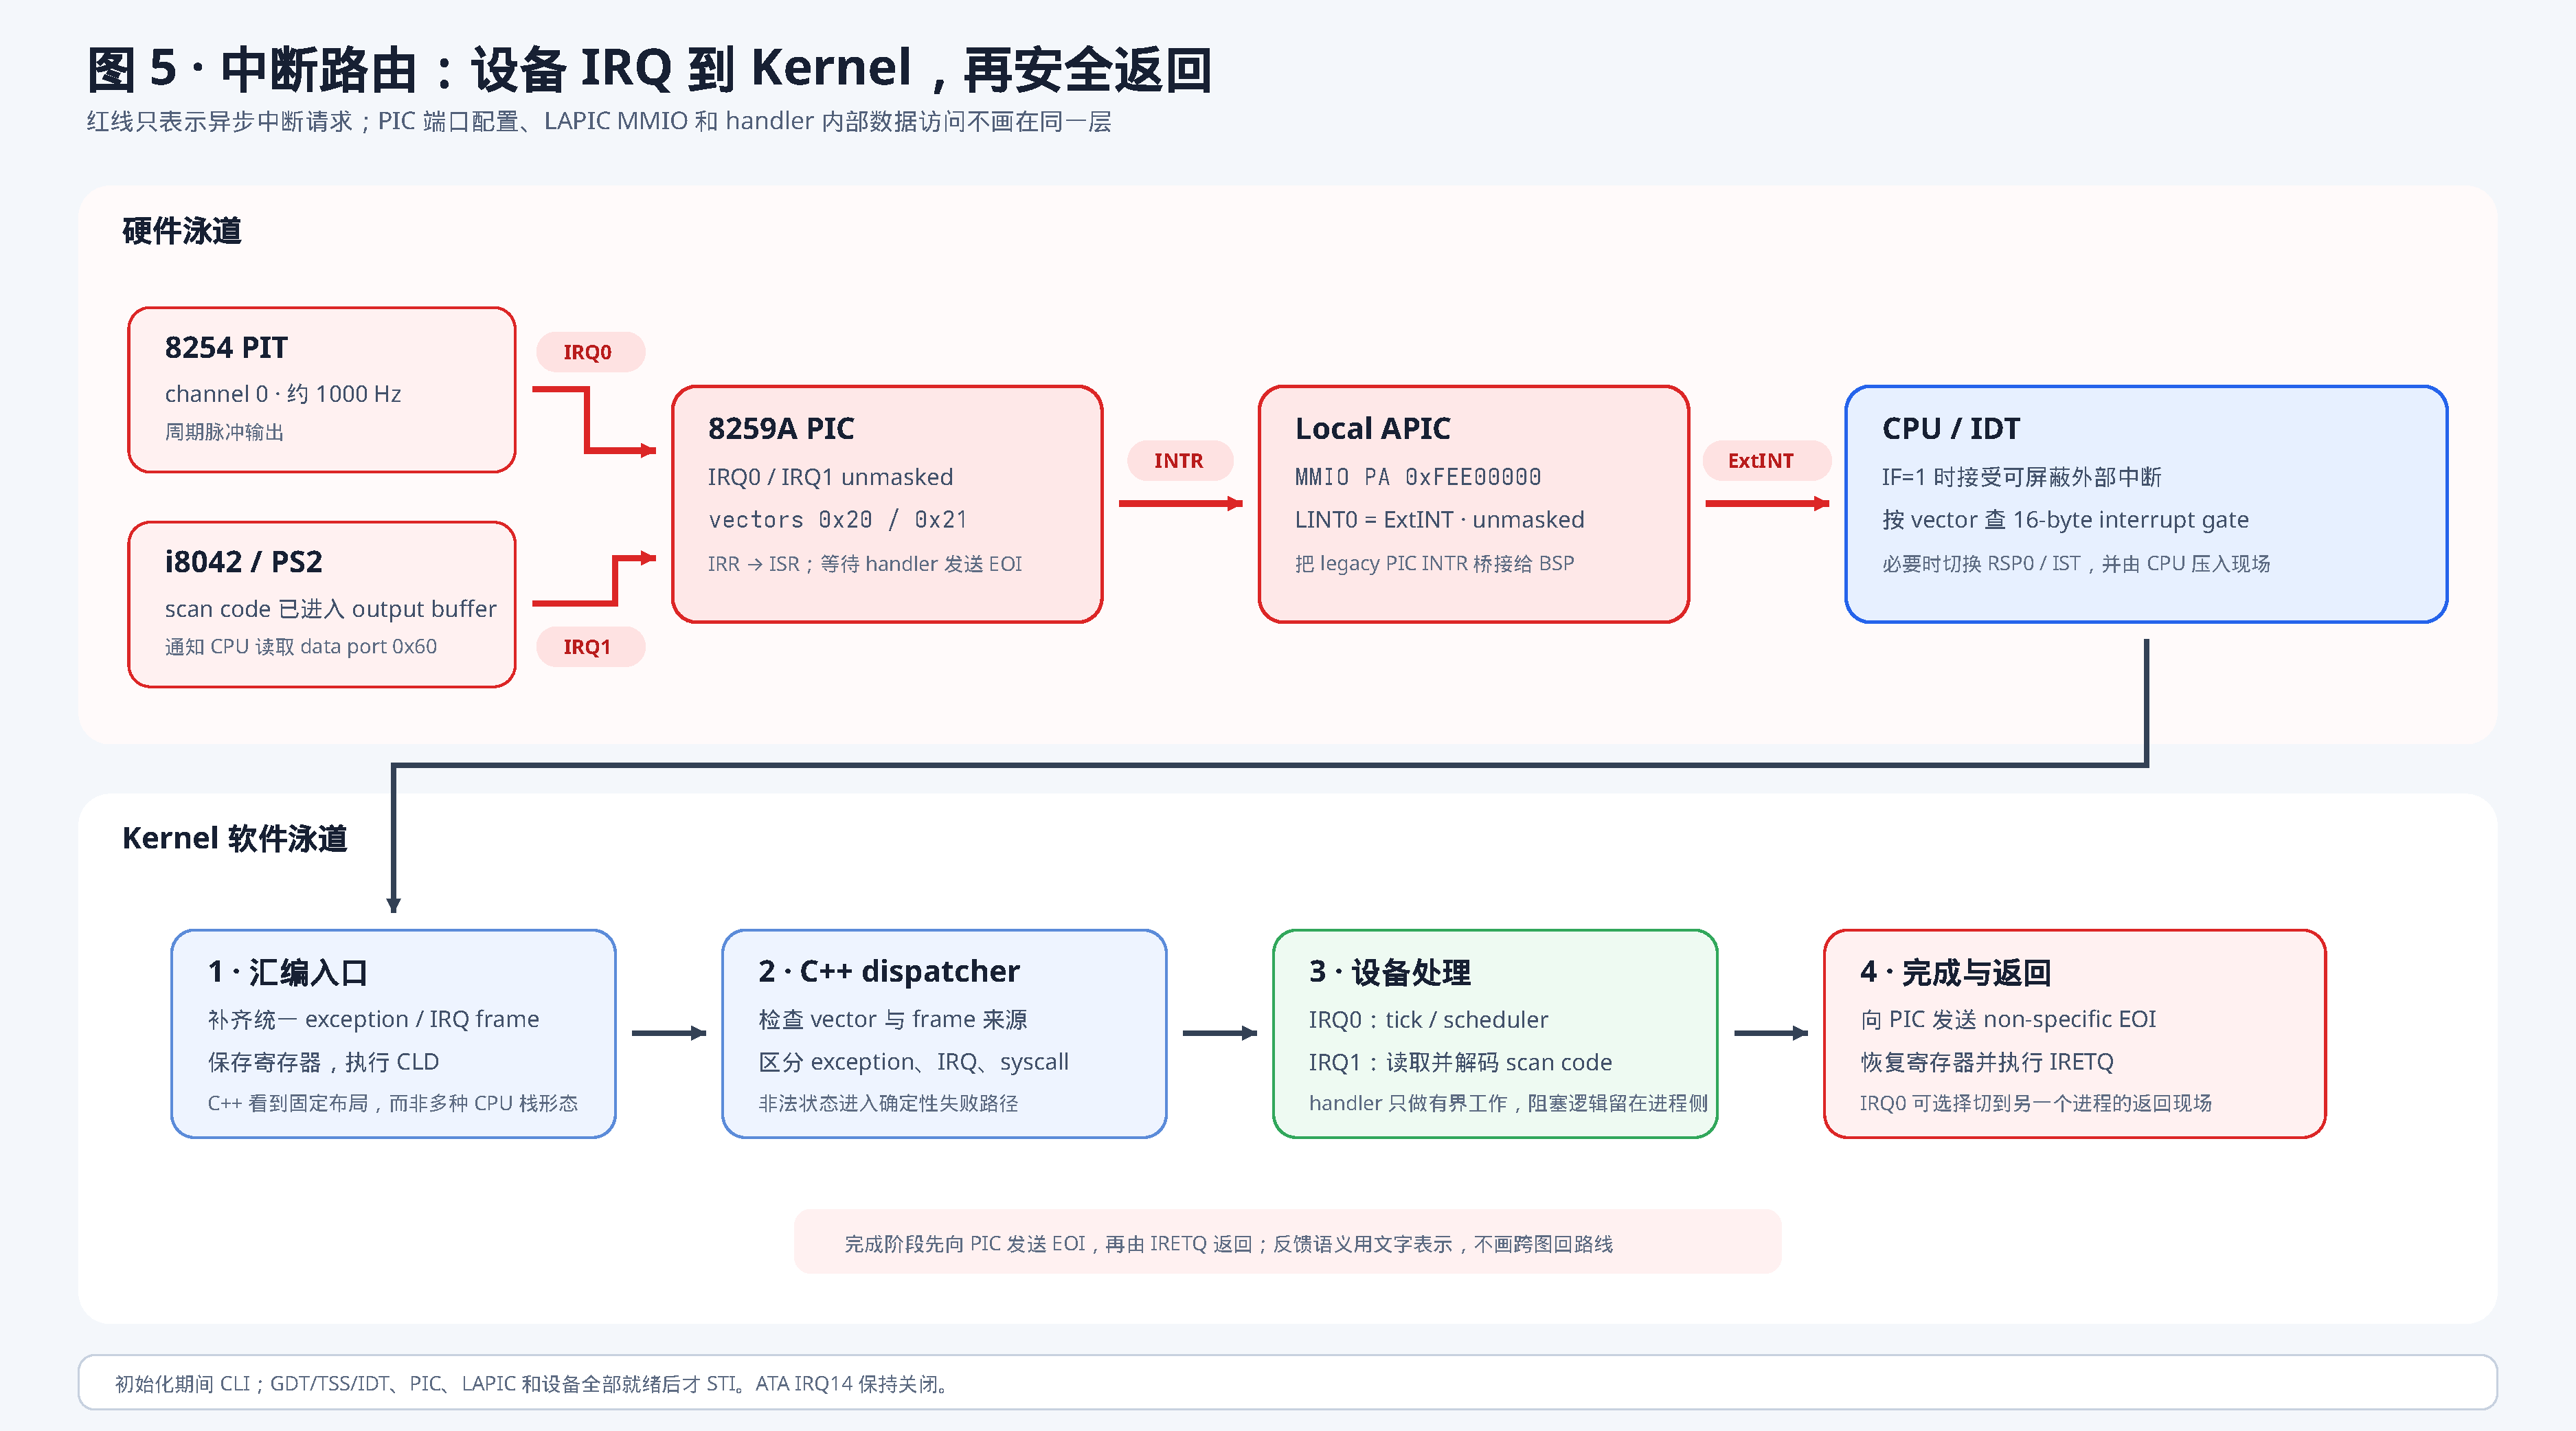
\includegraphics[width=0.96\textheight,height=0.82\textwidth,keepaspectratio]
    {figures/system_wiring/interrupt_routing.pdf}
  \caption{PIT/键盘的硬件 IRQ 经 8259A PIC 和 Local APIC 到达 CPU，再由
  汇编入口、C++ 分派、设备处理和 EOI/IRETQ 完成闭环。上半页红线是通知，
  下半页深色箭头是软件控制流，不能混成“设备直接调用 handler”。}
  \label{fig:interrupt-routing-full}
\end{sidewaysfigure}
\clearpage

\topic{一、IRQ 和 vector 为什么不是同一个编号}
\term{IRQ}{Interrupt Request，中断请求}是设备/控制器一侧的输入编号，例如
PIT 接 PIC IRQ0、键盘控制器接 IRQ1。\term{vector}{中断向量}是 CPU 用来索引
IDT 的 0--255 编号。PIC 初始化时建立映射，因此 IRQ0 可被交付为 vector
\code{0x20}，IRQ1 可被交付为 vector \code{0x21}。

必须重映射的原因是 CPU 低向量已经保留给架构异常。如果 PIC 延续早期默认范围，
设备 IRQ 会与除零、保护错误等异常编号重叠，handler 便无法仅凭 vector 判断
来源。重映射改变软件可见向量，不改变 PIT 仍连在 IRQ0 这条硬件事实。

\begin{osgridlongtable}{L{0.16\linewidth}L{0.24\linewidth}L{0.27\linewidth}L{0.23\linewidth}}
名称 & 所在层 & 本图例子 & 谁配置或产生 \\ \hline
IRQ line & 设备到中断控制器的请求 & IRQ0、IRQ1 & PIT/i8042 产生，PIC 接收 \\ \hline
PIC vector & 控制器交给 CPU 的编号 & \code{0x20}、\code{0x21} & Kernel 初始化 PIC offset \\ \hline
IDT entry & CPU 按 vector 找到的 16 B gate & entry 32、33 & Kernel 构造并 \code{lidt} \\ \hline
handler & 保存现场后运行的软件 & timer/keyboard C++ 分派 & 汇编 adapter 调用 \\ \hline
\end{osgridlongtable}

\topic{2.1 PIT 和 i8042 先保存各自的事件事实}
PIT channel 0 到期时产生周期脉冲；i8042 在 output buffer 已有扫描码时产生
IRQ1。红线只携带“请处理”的请求，不携带 tick 数字或扫描码字节。timer handler
通过已知设备语义增加软件 tick；keyboard handler 还必须从 port
\code{0x60} 读取控制器保存的数据。

\topic{2.2 PIC 仲裁、记录并等待 EOI}
PIC 的 IRR 记录待处理请求，IMR 决定哪些输入被屏蔽，ISR 记录已经交付但尚未
完成的请求。它按优先级选择 IRQ，输出 INTR。CPU 接受并应答后，PIC 提供
映射后的向量。handler 完成时发送 EOI，PIC 才能从 in-service 状态释放对应
层级。

EOI 太早可能让同源事件在共享状态尚未稳定时重入；EOI 太晚或遗漏则可能阻塞
后续中断。级联从片 IRQ 还涉及从片和主片的正确确认顺序。本项目当前只放行
主片 IRQ0/IRQ1，但驱动仍明确遵循完成协议。

\topic{2.3 Local APIC virtual-wire 是兼容桥}
Local APIC 位于 CPU 一侧，LINT0 配成 ExtINT 后，可把 legacy PIC 的 INTR
桥接给 BSP。这条路径叫 virtual wire，不表示它是“假的中断”；它是现代 APIC
体系承接传统 PIC 的兼容模式。Local APIC 自身通过 MMIO 配置，不在 Port I/O
图的蓝色总线上。

\topic{2.4 CPU 还要经过四道接收条件}
普通可屏蔽中断到达 handler，至少需要：

\begin{enumerate}[leftmargin=2.2em]
  \item 设备启用对应事件并真正提出 IRQ；
  \item PIC 没有在 IMR 屏蔽该输入，且路由/级联状态有效；
  \item Local APIC 的 LINT0/ExtINT 路径有效；
  \item CPU 的 RFLAGS.IF 为 1，IDT 对应 gate present 且入口可执行。
\end{enumerate}

所以“执行过 \code{sti}”不是完整证明。任何上游门关闭都不会进入 handler；
反过来，异常和 NMI 另有规则，也不会因为 IF 清零而全部消失。

\topic{三、CPU/IDT 如何安全改变控制流}
\term{IDT gate}{中断描述符表门}给出目标代码段、入口偏移、gate 类型、DPL、
present 位和可选 IST 编号。CPU 接受事件后按规范保存返回现场；跨特权级时
还要切到 TSS.RSP0 或指定 IST 栈。这个过程由硬件约束，设备不能任意指定内核
函数指针。

本项目的汇编入口把“CPU 有时压 error code、有时不压”的不同异常/IRQ 形态
规范成固定 C++ 可读 frame，保存 15 个通用寄存器并执行 \code{cld}。调用
C++ 前还要满足 System V AMD64 栈对齐。handler 看到的是经 adapter 明确定义的
数据结构，不是可以随意改字段顺序的普通函数参数。

\topic{四、Kernel 软件泳道的四个提交点}\par
\begin{osgridlongtable}{L{0.16\linewidth}L{0.27\linewidth}L{0.30\linewidth}L{0.17\linewidth}}
阶段 & 必须完成 & 失败边界 & 提交证据 \\ \hline
汇编入口 & 保存/规范化现场，建立 ABI 栈 & 任何调用前，不可破坏原现场 & 固定 frame 可审计 \\ \hline
C++ dispatcher & 检查 vector、来源与当前上下文 & 未知/非法状态走确定性失败 & 选中唯一 handler \\ \hline
设备处理 & 读取事实，更新最小有界状态 & 不在 IRQ 中无限等待或做阻塞用户工作 & tick/扫描码入队 \\ \hline
完成返回 & 按来源发送 EOI，恢复现场，\code{iretq} & 不得返回失效进程/栈 & 下一现场继续执行 \\ \hline
\end{osgridlongtable}

IRQ0 可能在返回时切换到另一个进程的保存现场，因此“返回”不一定回到被打断
进程；但无论选择哪个现场，都必须具有正确 CR3、Ring 0 栈、用户 frame 与资源
所有权。调度决定属于内核策略，IRETQ 只按给定合法现场执行硬件恢复。

\begin{sidewaysfigure}[p]
  \centering
  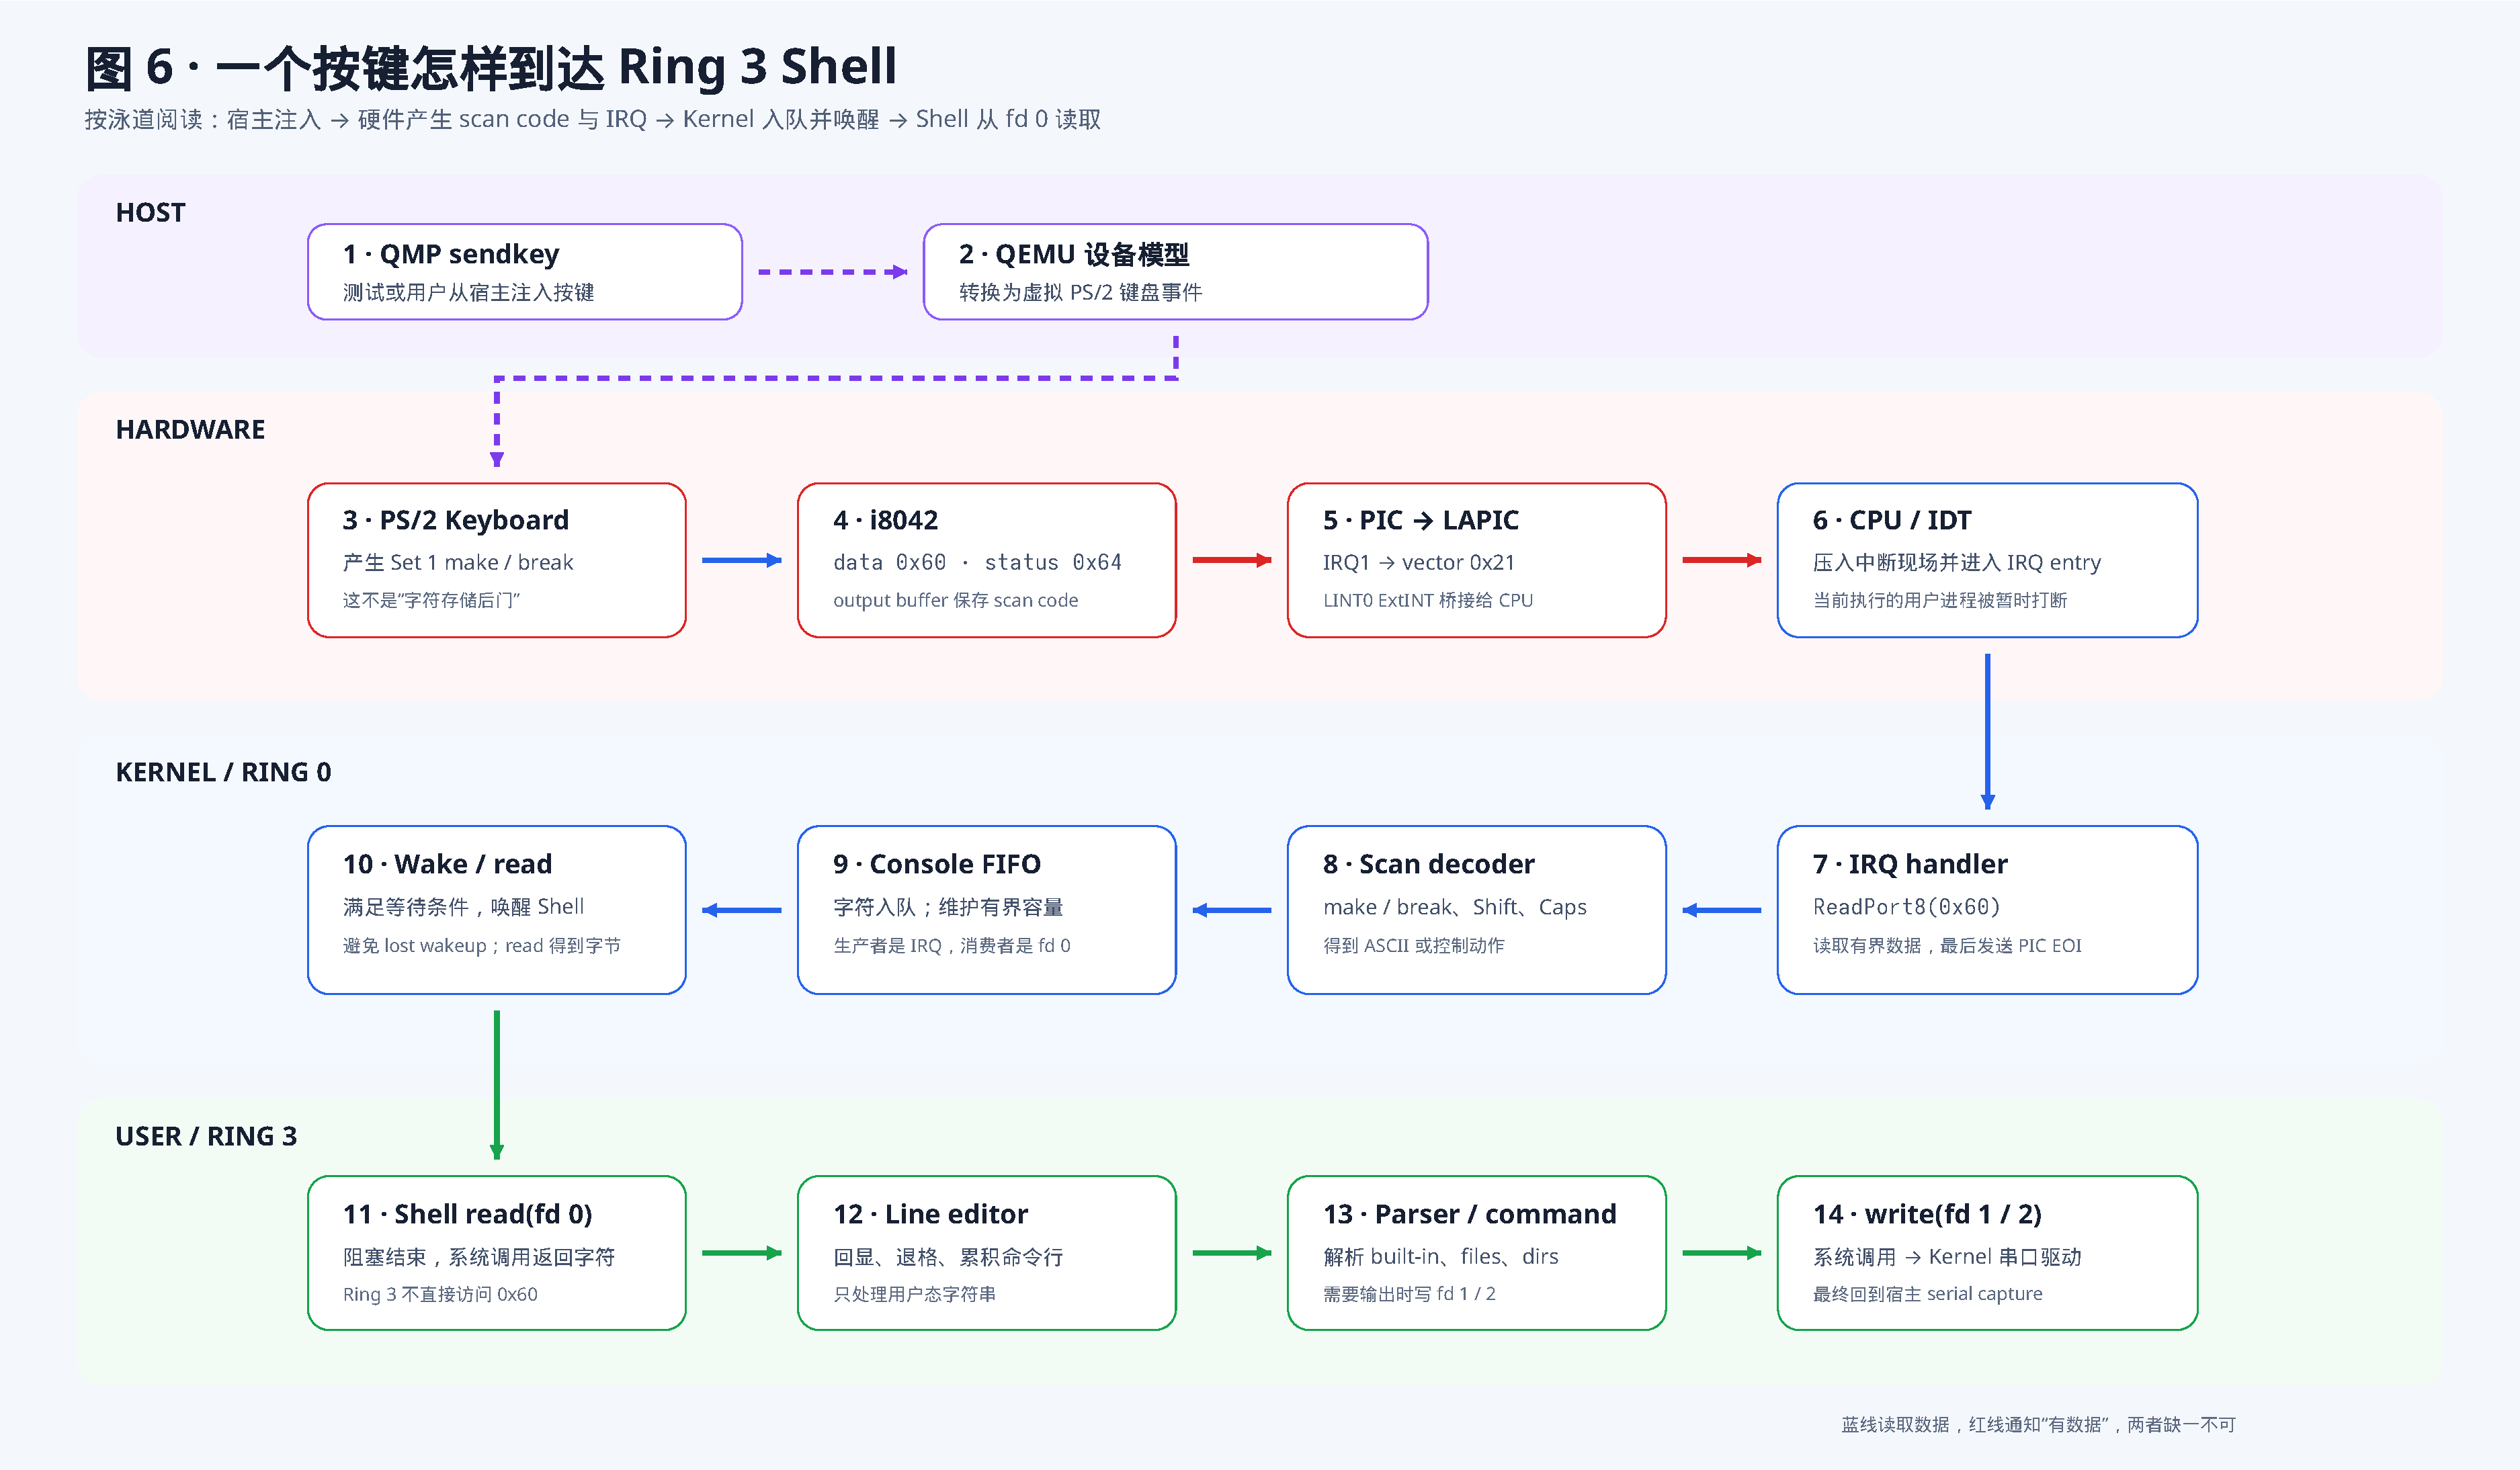
\includegraphics[width=0.96\textheight,height=0.82\textwidth,keepaspectratio]
    {figures/system_wiring/keyboard_to_shell.pdf}
  \caption{一个按键从宿主 QMP、QEMU PS/2 设备、IRQ1、Kernel FIFO 到 Ring 3
  Shell 的十四步路径。紫线是宿主注入，红线是 IRQ 通知，蓝线是内核数据流，
  绿线是用户态处理；不同颜色的箭头不可互换。}
  \label{fig:keyboard-to-shell-full}
\end{sidewaysfigure}
\clearpage

\topic{5.1 步骤 1--2：宿主请求不等于 Guest 字符}
自动化测试通过 QMP \code{sendkey} 向 QEMU 提交按键动作。QEMU 设备模型把它
转换成虚拟 PS/2 键盘事件。宿主传入的是控制命令，不是直接写入 Ring 3
缓冲区；QMP 与 Guest 的内存、端口和系统调用没有共用函数调用栈。

\topic{5.2 步骤 3--4：键盘产生扫描码，i8042 保存字节}
PS/2 键盘产生 Set 1 make/break 序列。i8042 把扫描码放进 output buffer，
状态端口 \code{0x64} 报告可读，数据端口 \code{0x60} 返回字节。按下 A 与
松开 A 是不同序列；Shift/Caps 状态也必须由后续解码器记忆，不能把每个字节
直接强制转换为 ASCII。

\topic{5.3 步骤 5--7：通知抵达，handler 才读取数据}
IRQ1 经 PIC 和 Local APIC 变成 vector \code{0x21}。CPU 保存现场并进入
IRQ entry；handler 再检查 i8042 状态并读取 \code{0x60}。顺序不能反过来：
没有读取数据寄存器，IRQ 线本身不会告诉 handler 是哪个键；没有正确中断路由，
缓冲区即使有数据也不会异步唤醒软件。

\topic{5.4 步骤 8--10：扫描码成为有界字符队列}
scan decoder 组合 make/break、扩展前缀、Shift 和 Caps 状态，产出字符或控制
动作。ConsoleInput 使用固定容量 FIFO 保存结果；生产者是 IRQ 路径，消费者是
等待 fd 0 的进程。队列满时必须遵守明确丢弃/计数策略，不能越界写；由空变为
可读时唤醒满足条件的 waiter，不能无条件唤醒所有进程。

\term{lost wakeup}{丢失唤醒}发生在“检查为空”和“登记睡眠”之间若没有同一
受保护事务：数据可能恰在缝隙到达，生产者看不到 waiter，消费者随后永久睡眠。
本项目把 compare-and-block 与队列状态放进明确锁/调度协议，Shell 的 read
才不会偶发卡死。

\topic{5.5 步骤 11--14：系统调用把字符交给 Shell}
Shell 在 Ring 3 对 fd 0 发起 read。系统调用验证用户缓冲区、解析当前进程
FileTable、确认对象可读；无数据则按协议阻塞，有数据则从 FIFO 复制到用户页。
Ring 3 从不直接执行 \code{in 0x60}，否则会绕过设备所有权、并发和隔离。

line editor 处理回显、退格和行边界，parser 把整行分成命令与参数，built-in
再访问文件/目录。输出经 fd 1/2 回到 Kernel 串口对象，最终进入宿主 serial
capture。因此输入和输出是两条独立端到端路径，在 Shell 层才汇合。

\topic{六、怎样按症状定位断在哪一层}\par
\begin{osgridlongtable}{L{0.25\linewidth}L{0.30\linewidth}L{0.35\linewidth}}
现象 & 首先检查 & 原因 \\ \hline
QMP 成功但没有 IRQ1 & QEMU 设备选择、i8042 初始化、PIC IMR、LAPIC、IF & 宿主命令只证明注入请求被接受 \\ \hline
IRQ1 计数增加但无字符 & \code{0x64} 状态、\code{0x60} 读取、扫描码 decoder & 通知路径正常不等于数据解释正常 \\ \hline
字符入 FIFO 但 Shell 卡住 & waiter 登记、唤醒条件、调度、fd 0 对象 & 硬件路径已完成，故障位于阻塞协议 \\ \hline
Shell 收到错字符 & make/break、扩展前缀、Shift/Caps 状态 & 不能只检查 IRQ 数量 \\ \hline
能输入但无回显 & fd 1/2、系统调用返回、UART THRE 与 serial capture & 输出链独立于输入链 \\ \hline
第一个键后再无中断 & i8042 数据是否取走、PIC EOI 是否发送 & 设备/PIC 可能仍保持未完成状态 \\ \hline
\end{osgridlongtable}

\begin{failurebox}
中断 handler 的日志本身会改变时序，串口轮询甚至可能显著延长关中断窗口。
调试时先用计数器、固定标记和超时证明边界，热路径成功后移除逐事件日志；
最终证据应同时覆盖 IRQ 到达、数据守恒、无丢失唤醒、正确 EOI 和合法返回现场。
\end{failurebox}
